\documentclass[9pt]{beamer}
\usepackage[utf8]{inputenc}
\usepackage[T1]{fontenc}
%\usepackage{verdana} %?
\usepackage[russian]{babel}
\usepackage{graphicx}
\usepackage{tikz}
\usepackage{pifont}
\usepackage{amsmath}
\usepackage{mathtools}
\usetheme{Warsaw}
\usecolortheme{orchid}
\setbeamertemplate{frametitle}
{
    \begin{beamercolorbox}[sep=0.3cm,ht=2.2em,wd=\paperwidth]{frametitle}
        \vbox{}\vskip-2.0ex%
        \strut\insertframetitle\strut
        \vskip-0.8ex%
    \end{beamercolorbox}
}

%\renewcommand{\familydefault}{verdana}
\setbeamerfont{block title}{size=\normalsize}
\title[World development indicators]{\huge World development indicators}
\subtitle[Which country will develop more]{\large Which country will develop more}
\author[Moawad, Comandini, Isaeva, Schiavon, Snesarevskii] {{\Large Group 12:\\}Stefano Moawad\\Leonardo Comandini\\Diana Isaeva\\Andrea Schiavon\\Viktor Snesarevskii}
\date{April-May 2017}
\usebackgroundtemplate{\tikz\node[opacity=0.3] {\vbox to \paperheight{\vfil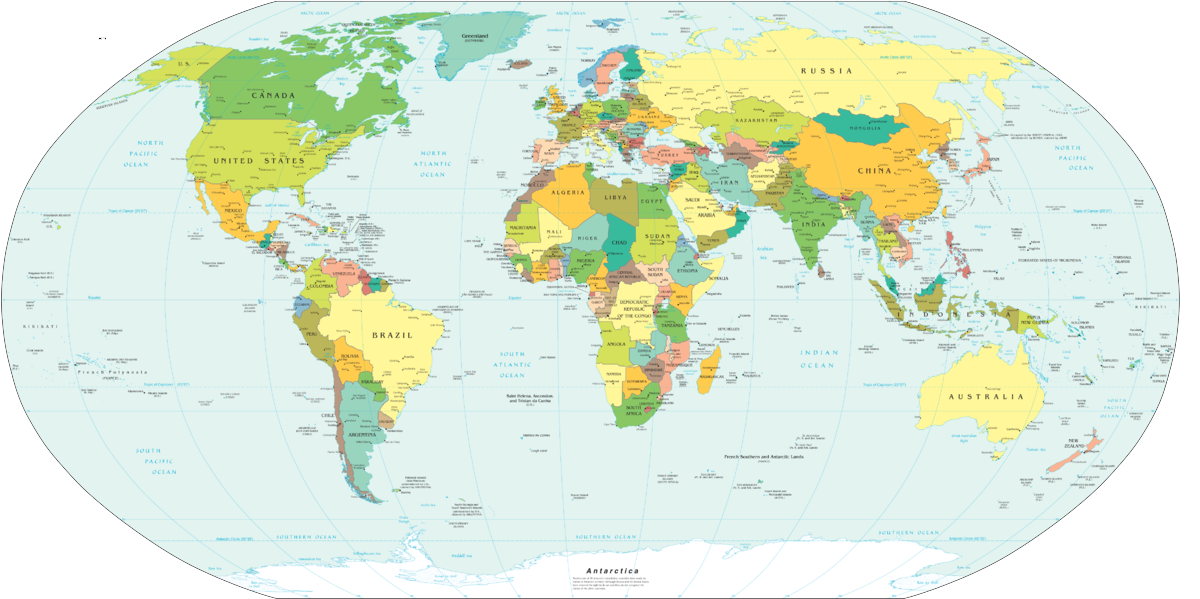
\includegraphics[width=\paperwidth]{map}\vfil}};}




\setbeamertemplate{headline}{}
\begin{document}
	\begin{frame}
	\titlepage
	\vfill
	\begin{flushright}
		
\includegraphics[height=.7cm]{kaggle.png}\quad
		
\includegraphics[height=.7cm]{worldbank.jpg}
	\end{flushright}
\end{frame}

% slide con tabella dei contenuti
\begin{frame}
	\frametitle{Table of Contents}
	\tableofcontents
\end{frame}


\section{Inference}

\subsection{growth}


\begin{frame}{What do economists mean by growth?}
	\begin{columns}[T] % contents are top vertically aligned
		\begin{column}[T]{5cm} % each column can also be its own environment
		\begin{definition}
		 by \alert{Growth} we mean the annual percentage variation of the GDP per capita in local currency. More formally,
		 \begin{equation}
		 Growth_{t} := \frac{GDP_{t}-GDP_{t-1}}{GDP_{t-1}}
		 \end{equation}
		 where $ GDP $ is the Gross Domestic Product per capita
		\end{definition}	
		\end{column}
		\begin{column}[T]{5cm} % alternative top-align that's better for graphics
			
\includegraphics[height=6cm]{economist-growth.jpg}
		\end{column}
	\end{columns}
\end{frame}


\begin{frame}{World economic growth from 1970 to 2010}
	\begin{block}{}
		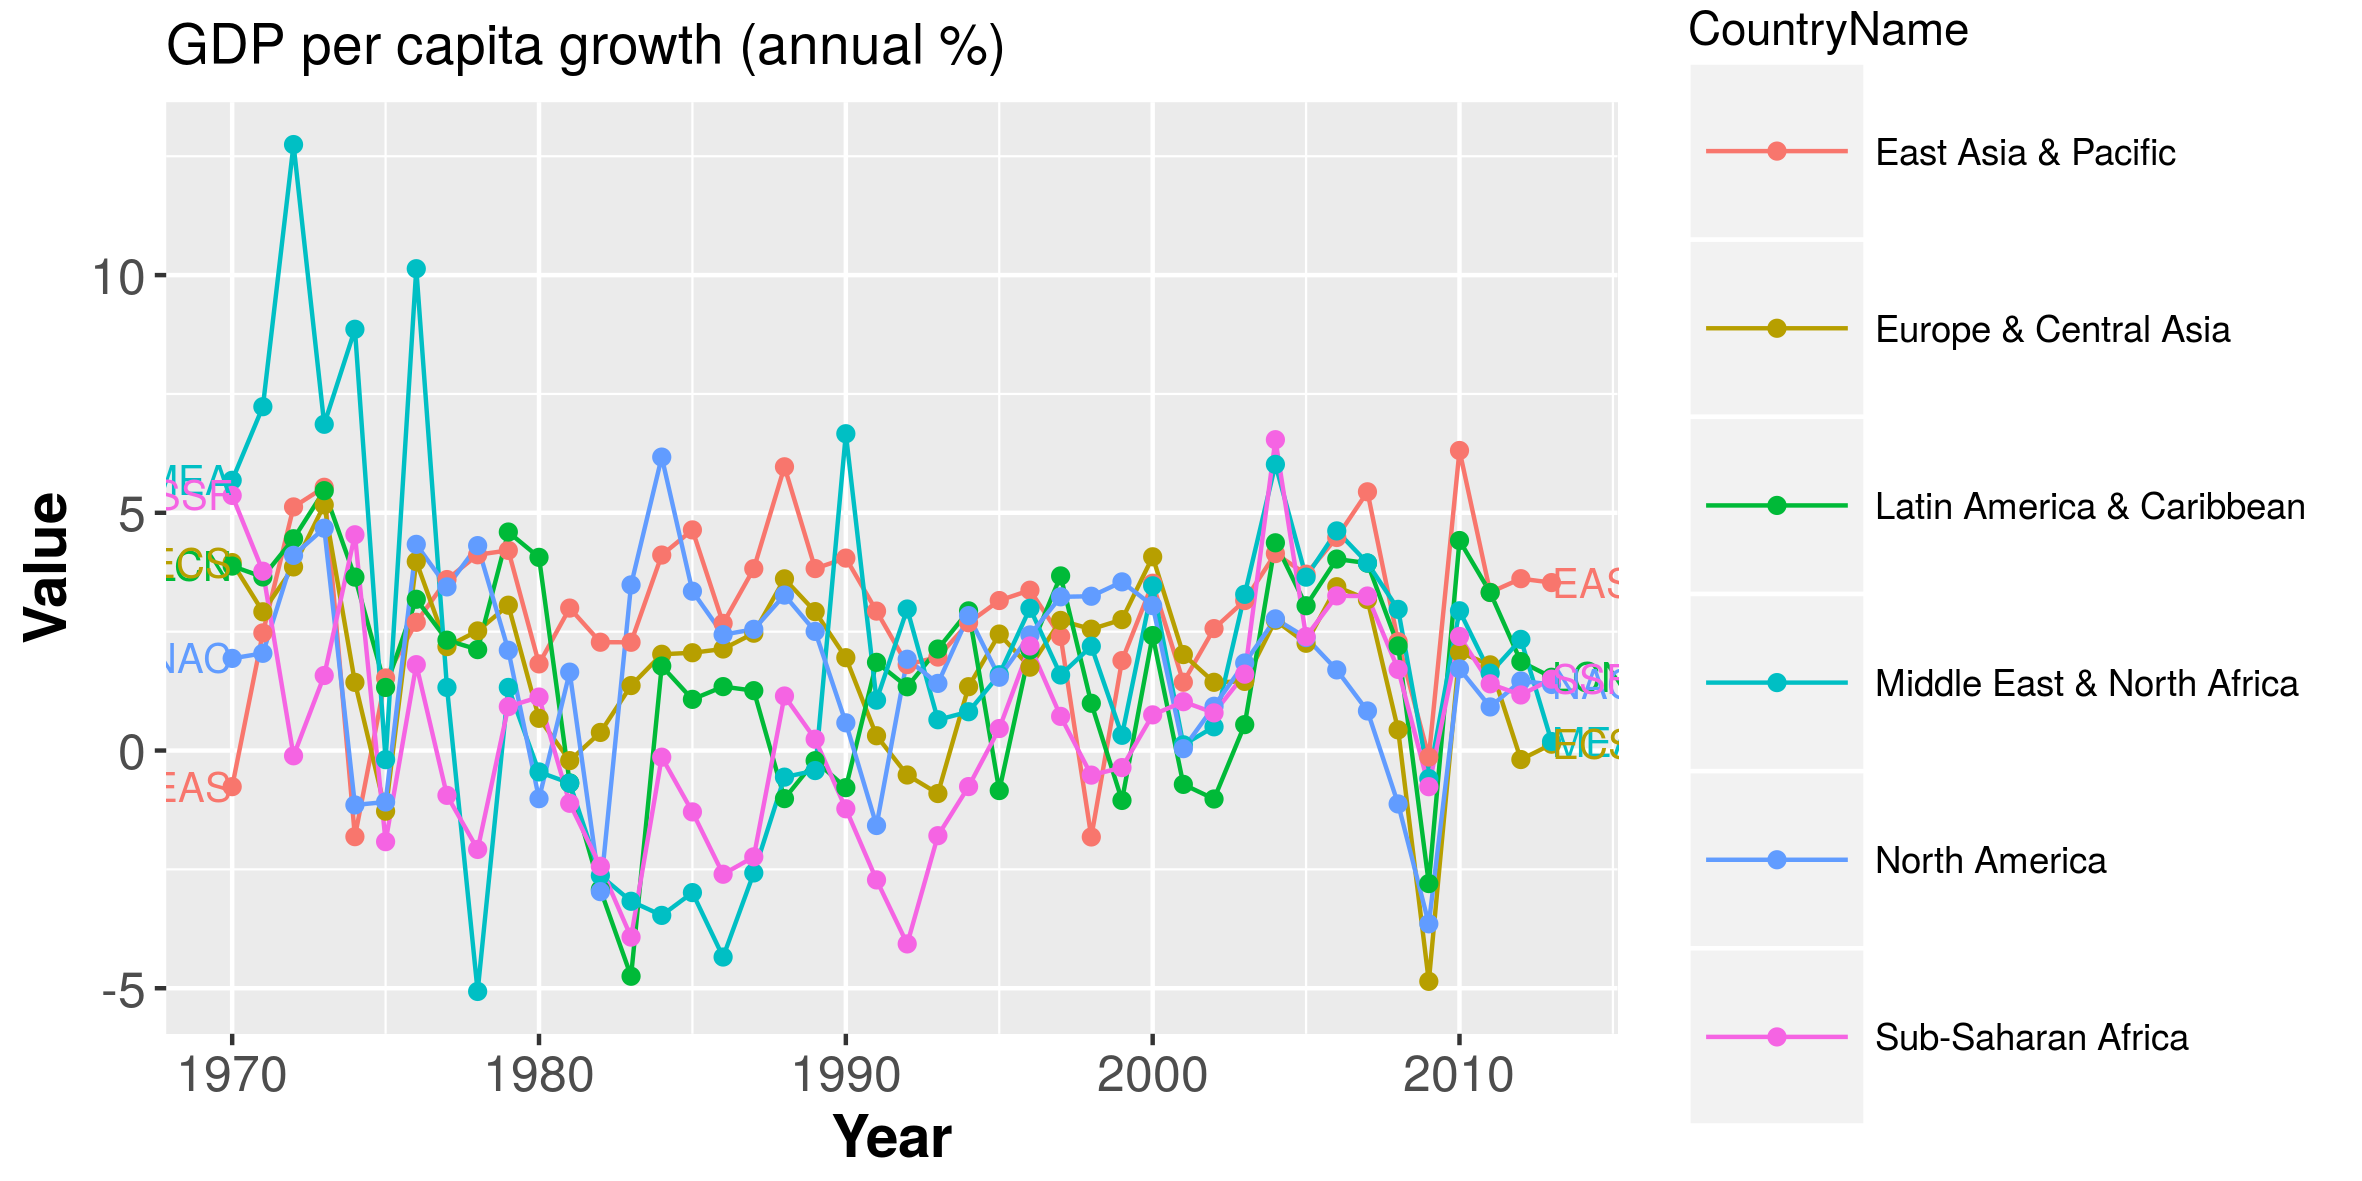
\includegraphics[height=5.5cm]{growth.png}
	\end{block}
	\begin{block}{questions}
		\begin{itemize}
			\item can we say that there was no growth over this time span?
			\item what happened in 2008/2009?
		\end{itemize}
	\end{block}
\end{frame}

\begin{frame}{T2 test}
	 % contents are top vertically aligned
		\begin{block}{} % each column can also be its own environment
			\[
			\begin{dcases}
				H_{0} \quad : \underline{\mu} = \underline{0} \implies  \text{no growth over the considered time span} \\
				H_{A} \quad : \underline{\mu} \ne \underline{0}
			\end{dcases}
			\]	
		\end{block}
		\begin{block}{} % alternative top-align that's better for graphics
			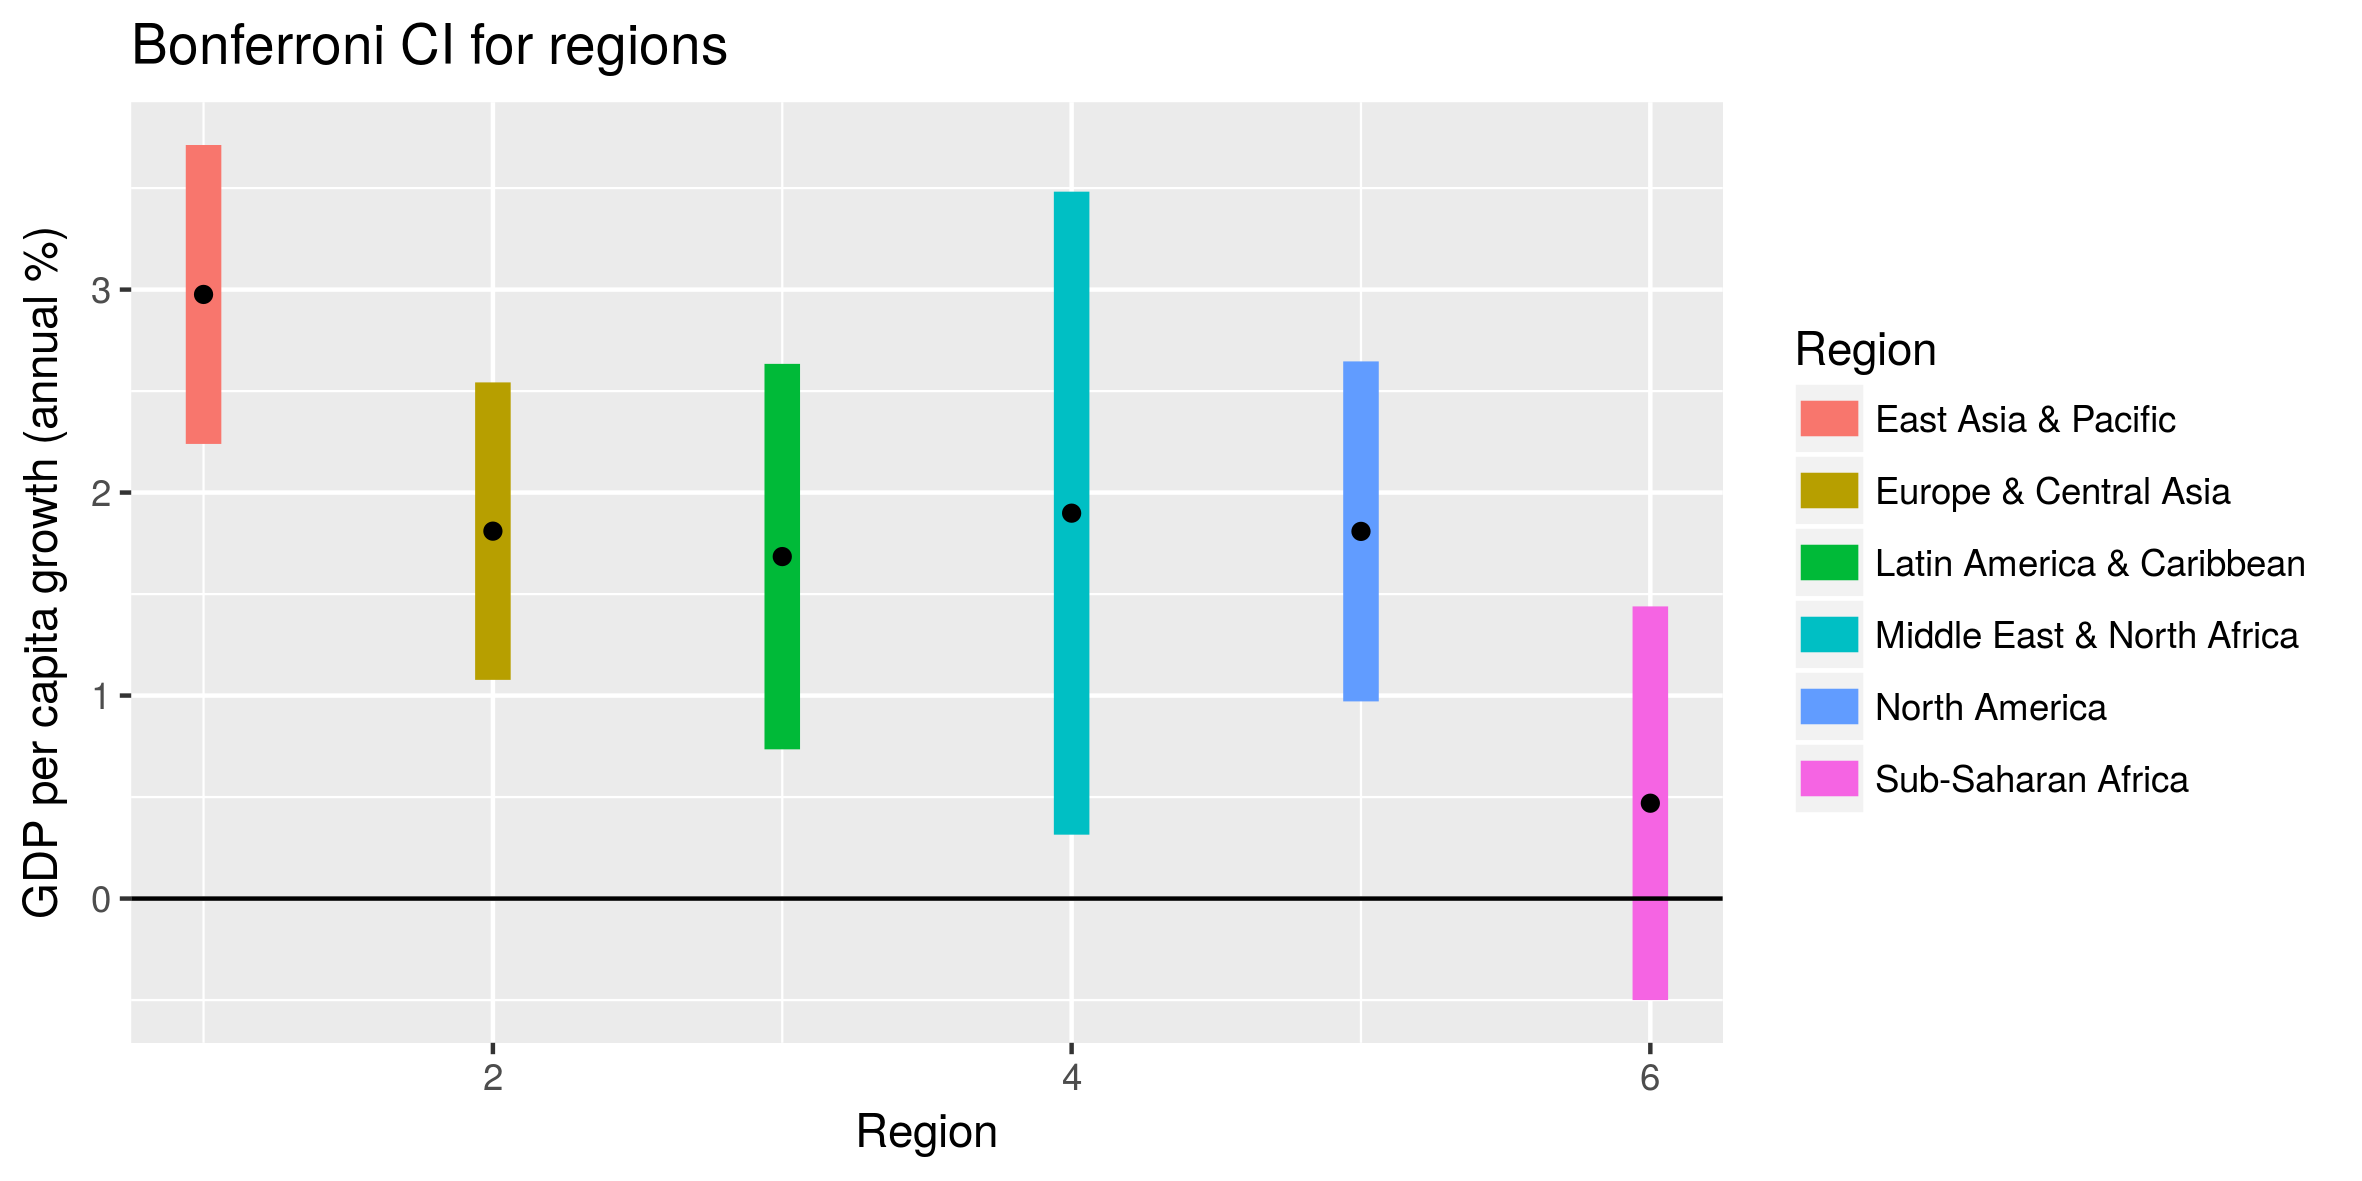
\includegraphics[height=6cm]{CI.png}
		\end{block}
\end{frame}

\subsection{growth during the 2008 crisis}

\begin{frame}{repeated measures test}
	% contents are top vertically aligned
	\begin{block}{} % each column can also be its own environment
		
%		\[
%		C = \begin{bmatrix}
%		1 & -1 & 0 \\
%		1 & 0  & -1
%		\end{bmatrix}
%		\]

		% setta il test con la graffa solita
		\[
		\begin{dcases}
		H_{0} \quad : C\underline{\mu} = \underline{0} \implies  \mu_{1} - \mu_{2} = 0  \quad\text{and}\quad \mu_1 - \mu_3 = 0 \\
		H_{A} \quad : C\underline{\mu} \ne \underline{0}
		\end{dcases}
		\]
		$ p.value = 0$	
	\end{block}
	\begin{block}{} % alternative top-align that's better for graphics
		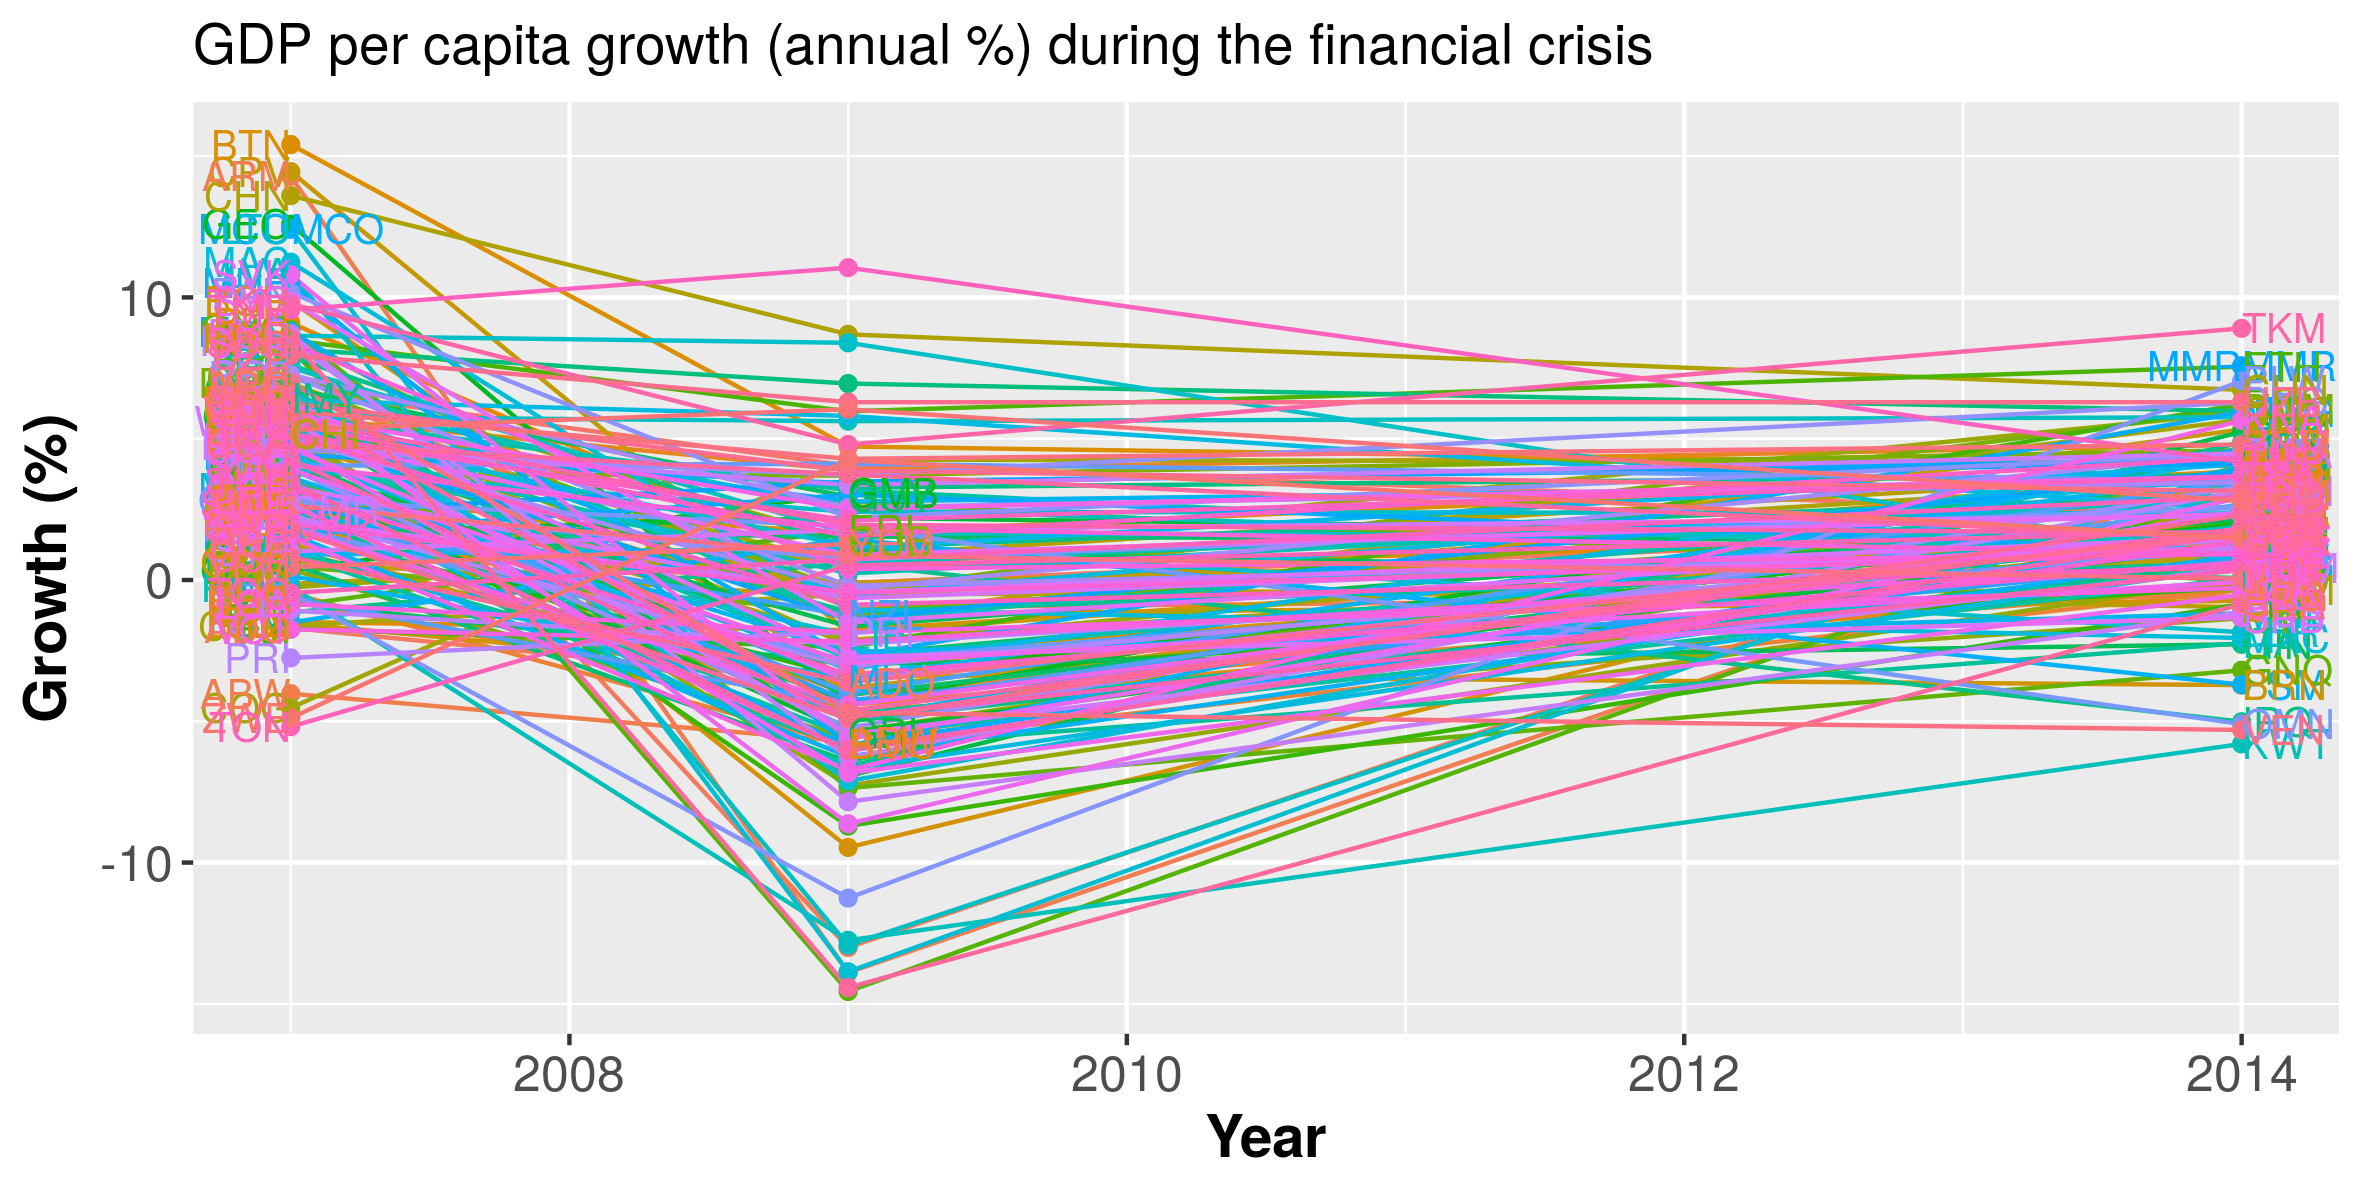
\includegraphics[height=5cm]{crisis.png}
	\end{block}
\end{frame}

\subsection{Growth vs Income, Region, and Year}

\begin{frame}{What affects growth?}
	\begin{block}{}
		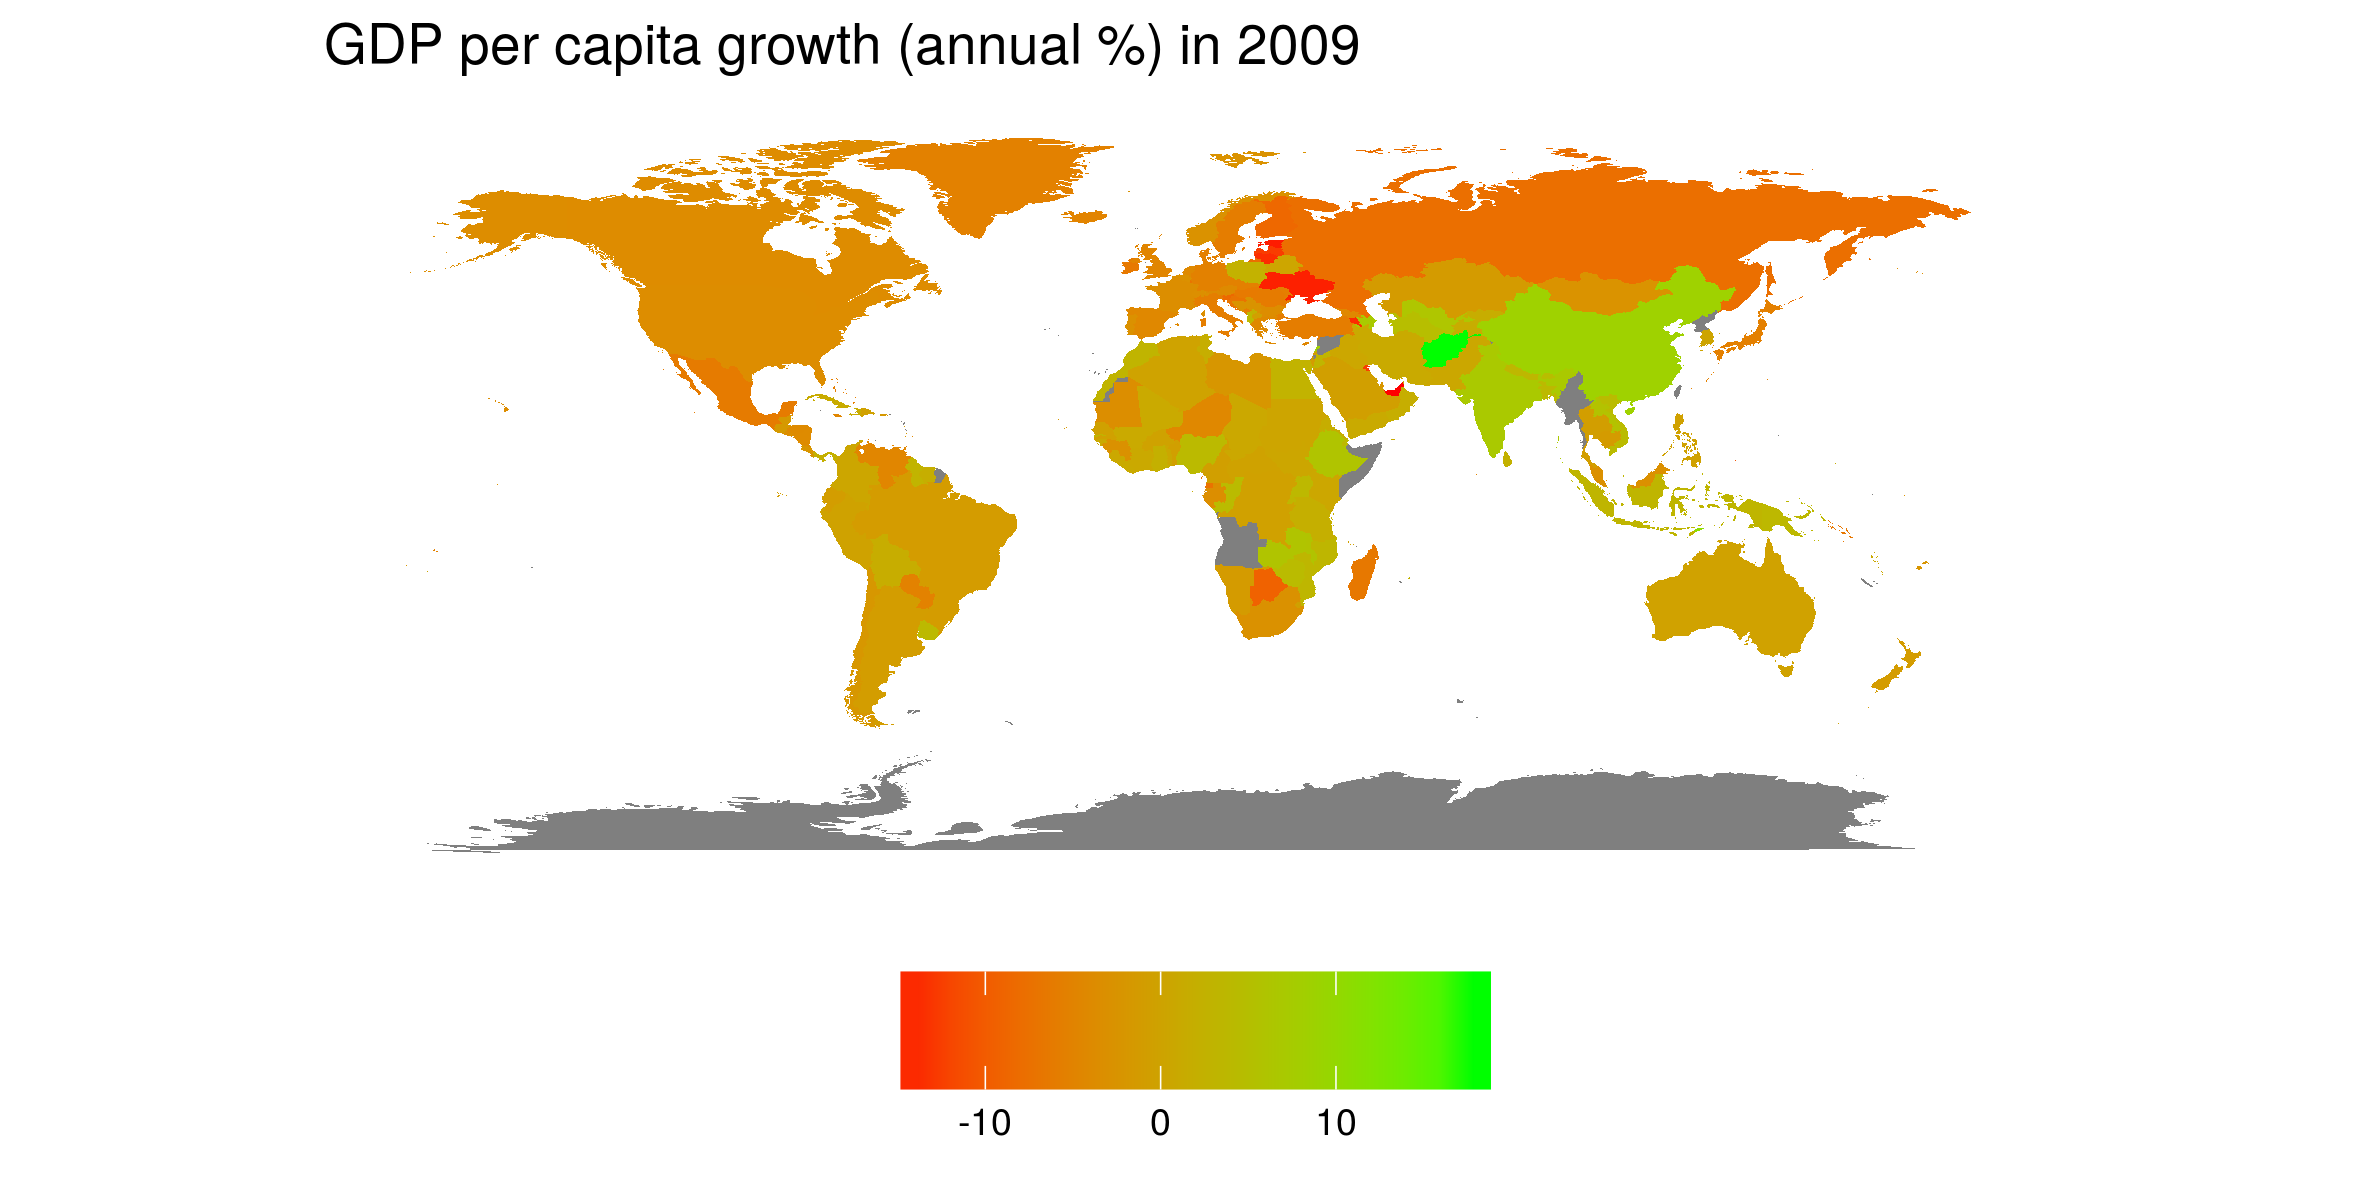
\includegraphics[height=5.5cm]{mappa.png}
	\end{block}
	\begin{block}{questions}
		\begin{itemize}
			\item during an economic crisis does geography play a role?
			\item does an economic crisis strike heavier high-income countries than low-income ones?
		\end{itemize}
	\end{block}
\end{frame}

%\begin{frame}{ANOVA two-way}
%	\begin{table}[ht]
%		\centering
%		\begin{tabular}{rrrrrrr}
%			\hline
%			& Asia & EU & Latin Am & Middle East & North Am & Africa \\ 
%			\hline
%			2007  \\ 
%			2009                & $ X_{ij}$  \\ 
%			2014  \\ 
%			\hline
%		\end{tabular}
%	\end{table}
%\end{frame}


\begin{frame}{ANOVA two-way}
	
	\begin{block}{during an economic crisis}
		Year = {[2007, 2009, 2014]}
		\begin{table}[ht]
			\centering
			\begin{tabular}{lrrrrr}
				\hline
				& Df & Sum Sq & Mean Sq & F value & Pr($>$F) \\ 
				\hline
				fRegion & 6 & 315.58 & 52.60 & 4.43 & 0.0002 \\ 
				Year & 2 & 3362.03 & 1681.01 & 141.59 & 0.0000 \\ 
				fRegion:Year & 12 & 894.73 & 74.56 & 6.28 & 0.0000 \\ 
				Residuals & 533 & 6328.06 & 11.87 &  &  \\ 
				\hline
			\end{tabular}
		\end{table}
	\end{block}
	
	\begin{block}{not economic turmoils}
		Year = {[2000, 2003, 2006]}
		\begin{table}[ht]
			\centering
			\begin{tabular}{lrrrrr}
				\hline
				& Df & Sum Sq & Mean Sq & F value & Pr($>$F) \\ 
				\hline
				fRegion & 6 & 875.35 & 145.89 & 7.37 & 0.0000 \\ 
				Year & 2 & 317.40 & 158.70 & 8.02 & 0.0004 \\ 
				fRegion:Year & 12 & 171.12 & 14.26 & 0.72 & 0.7318 \\ 
				Residuals & 556 & 11001.81 & 19.79 &  &  \\ 
				\hline
			\end{tabular}
		\end{table}
	\end{block}
\end{frame}


\begin{frame}{let's visualize the interaction}
	\begin{block}{}
		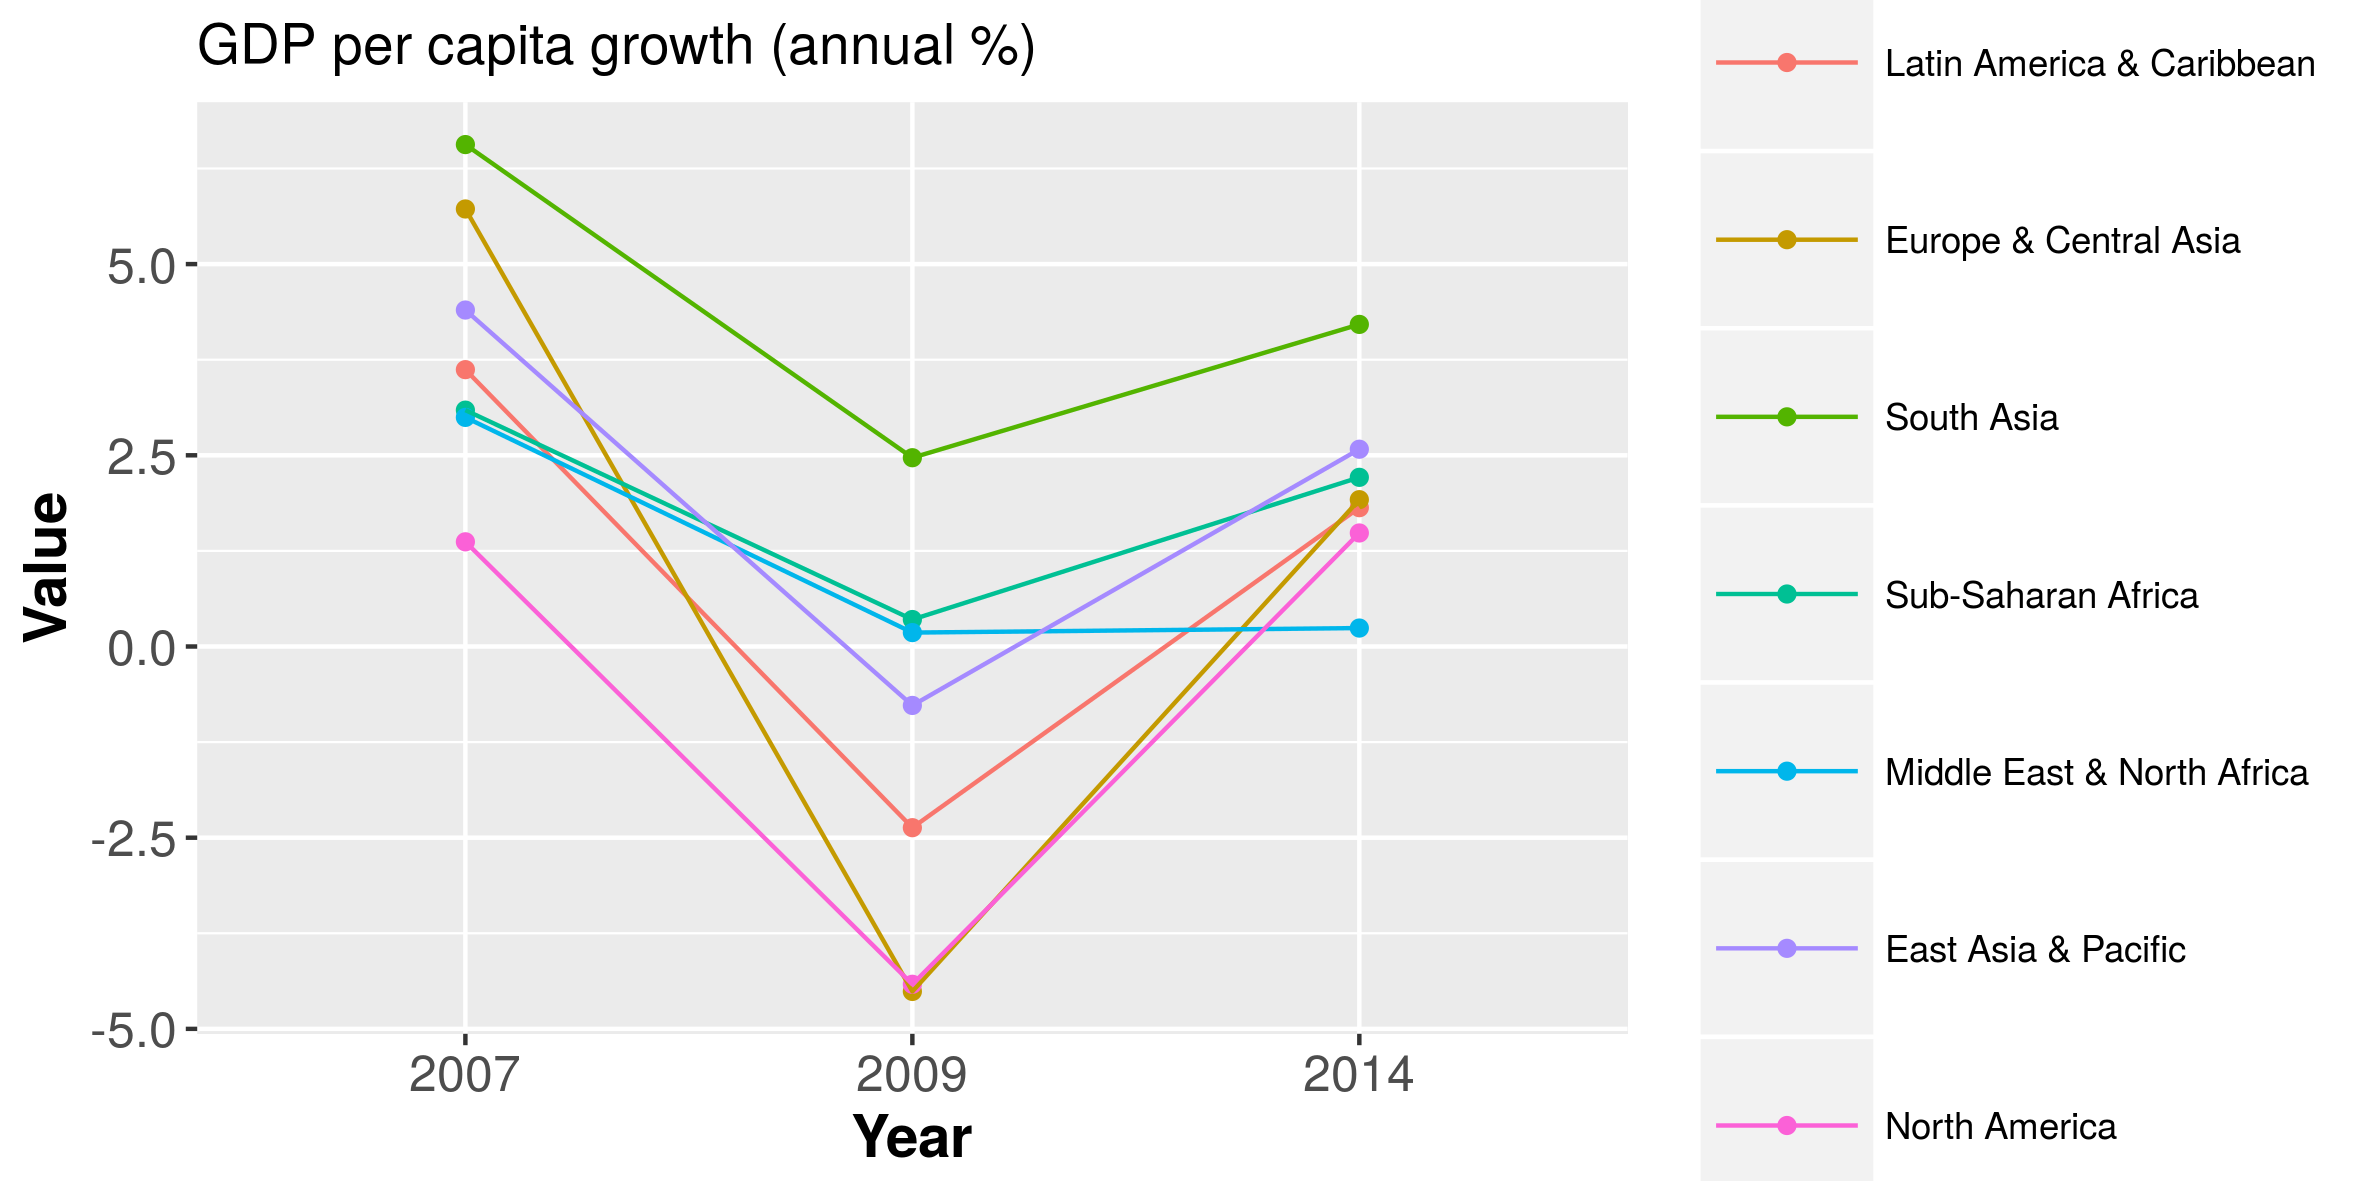
\includegraphics[height=3.8cm,width = 10cm]{inter1.png}
	\end{block}
	\begin{block}{}
		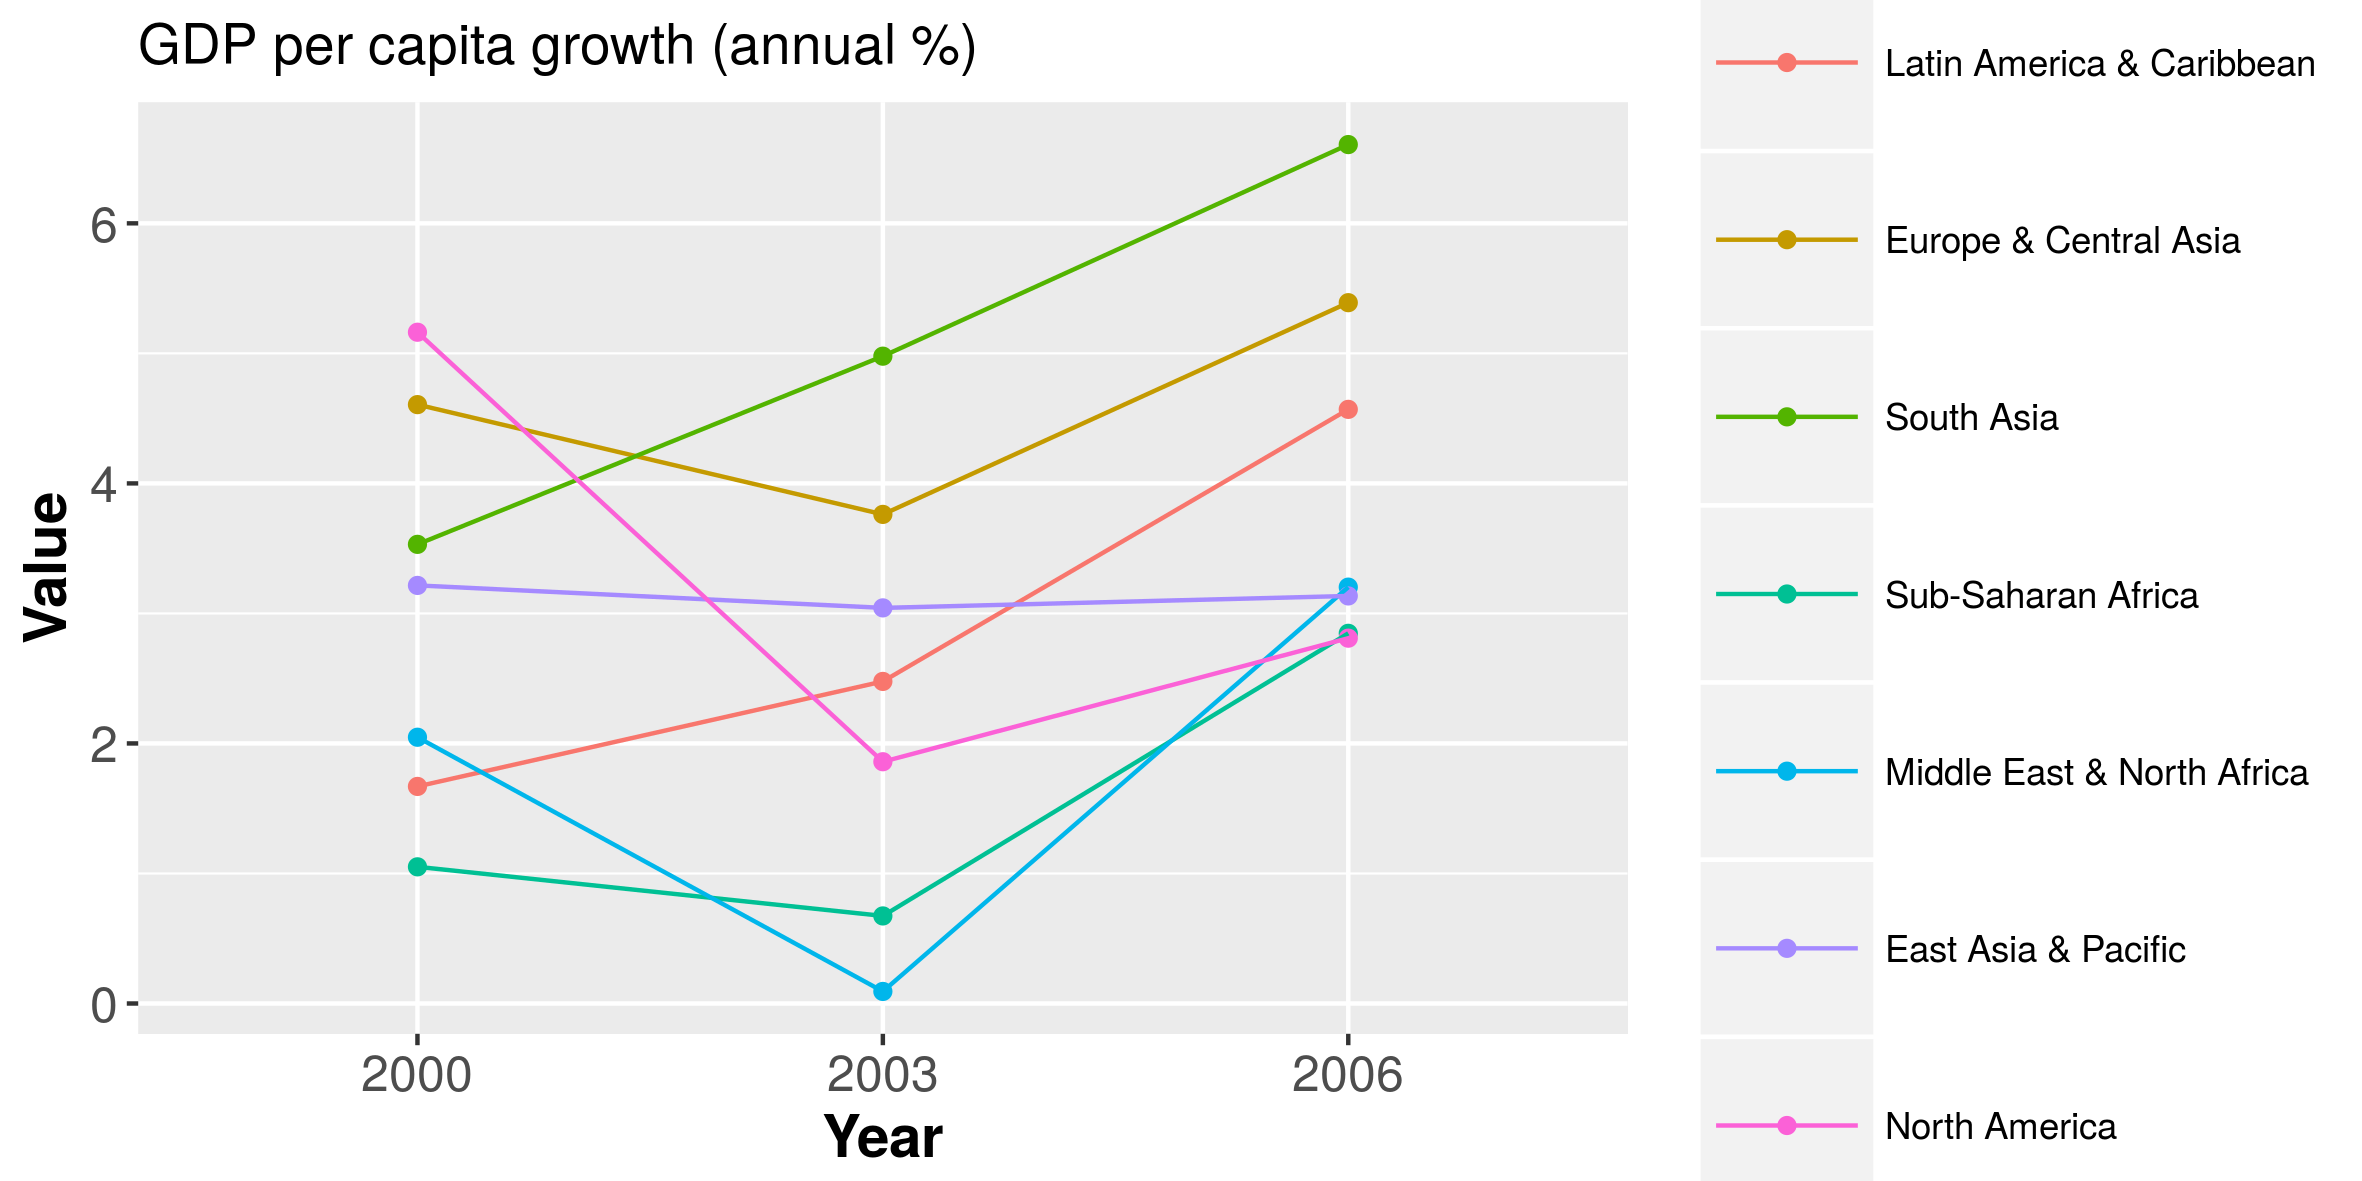
\includegraphics[height=3.5cm,width = 10cm]{inter2.png}
	\end{block}
\end{frame}


\begin{frame}{Does IncomeGroup affect Growth?}
	\begin{block}{}
		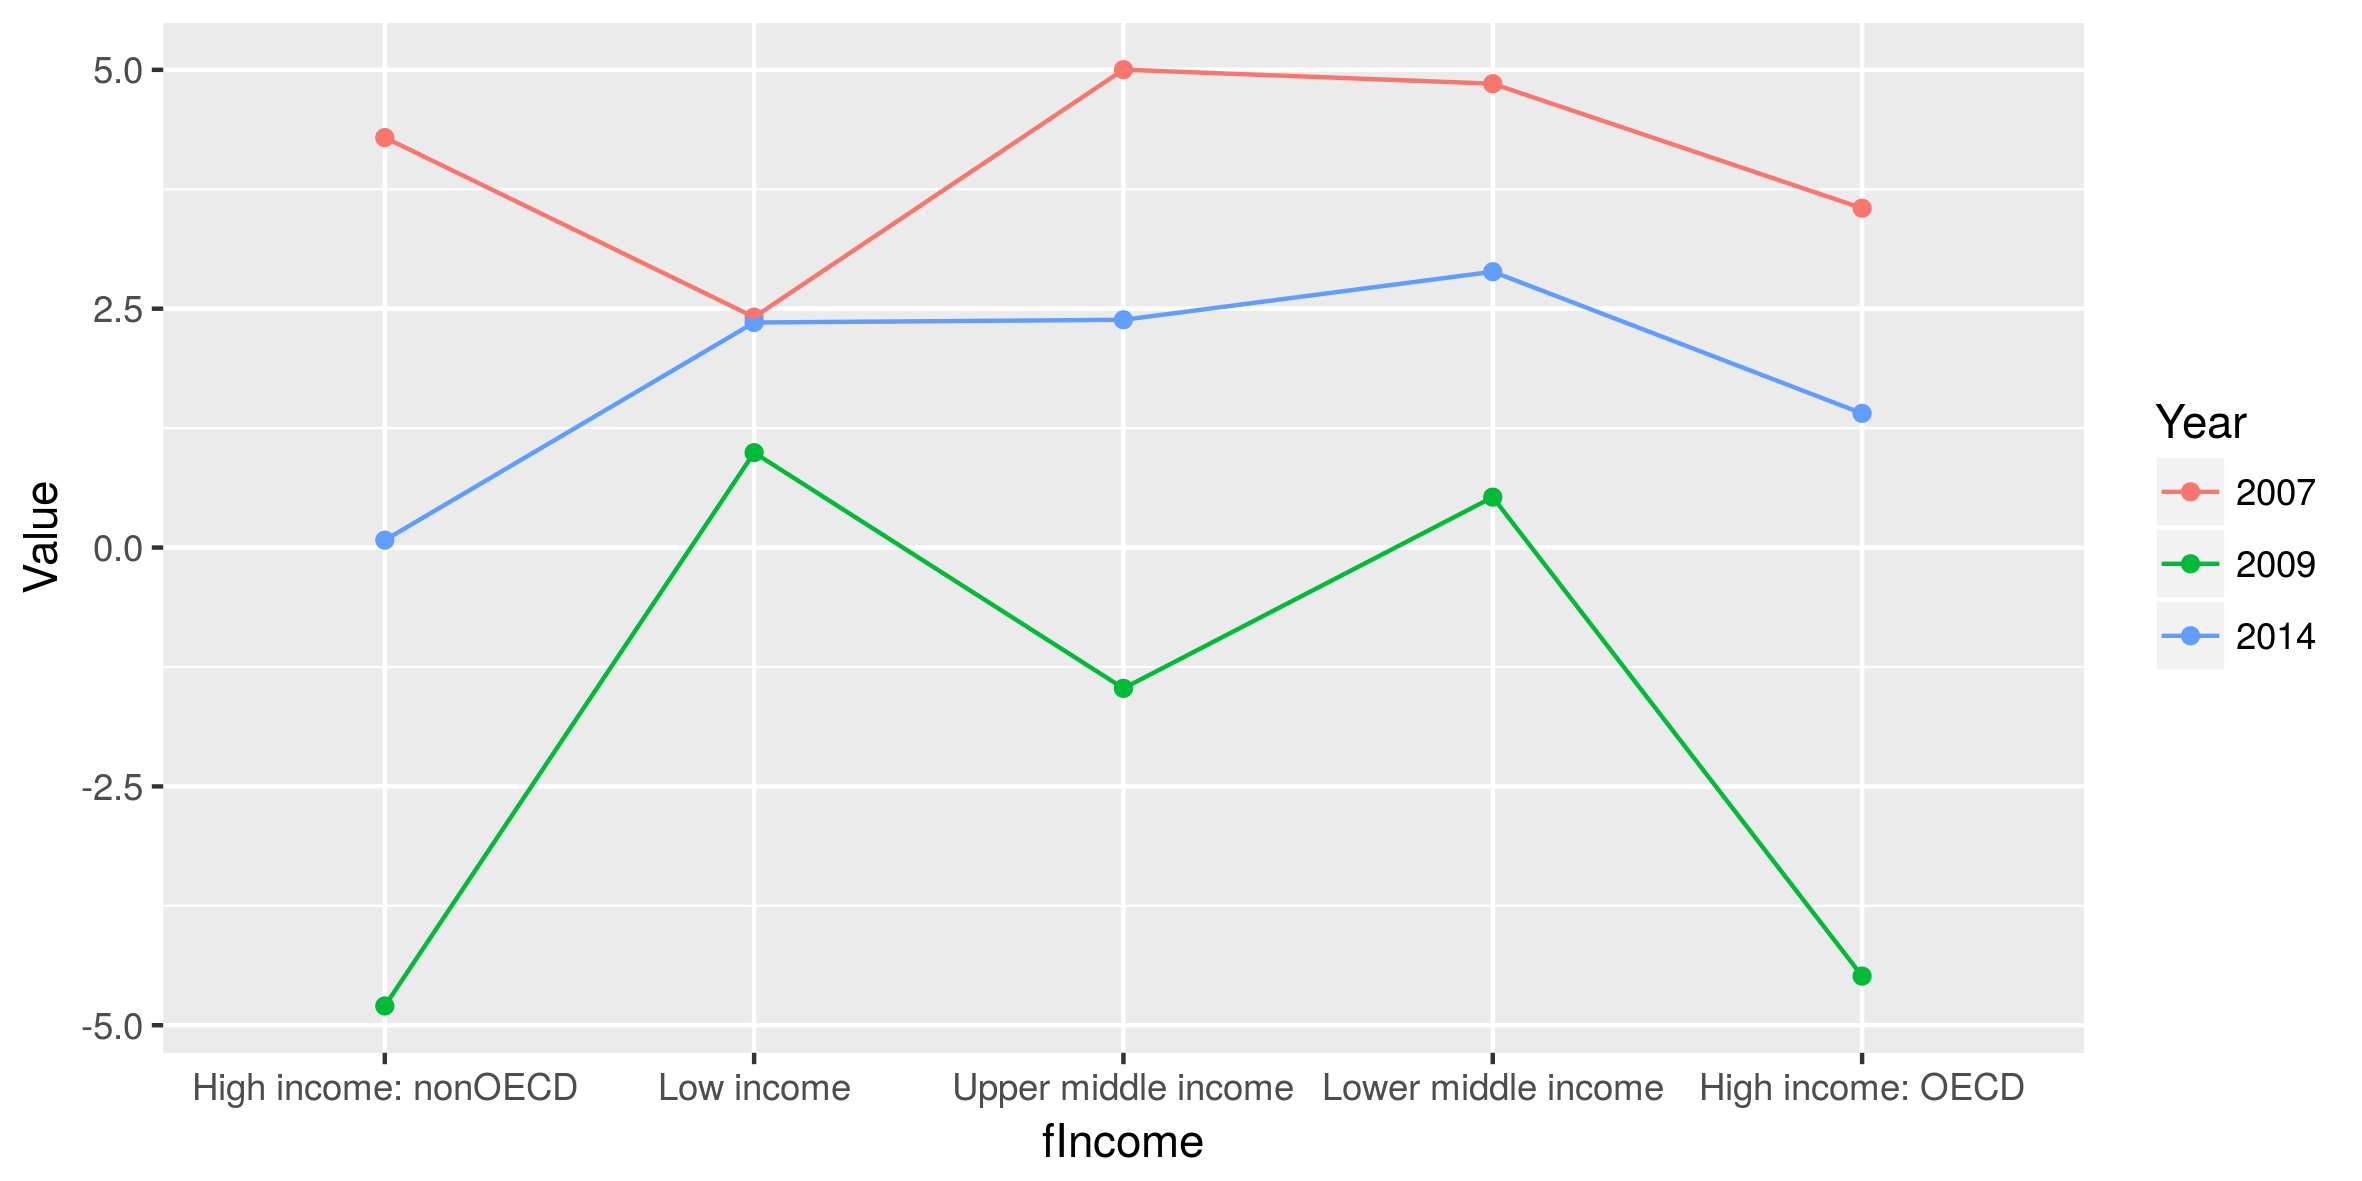
\includegraphics[height=3.8cm,width = 10cm]{Income1.png}
	\end{block}
	\begin{block}{}
		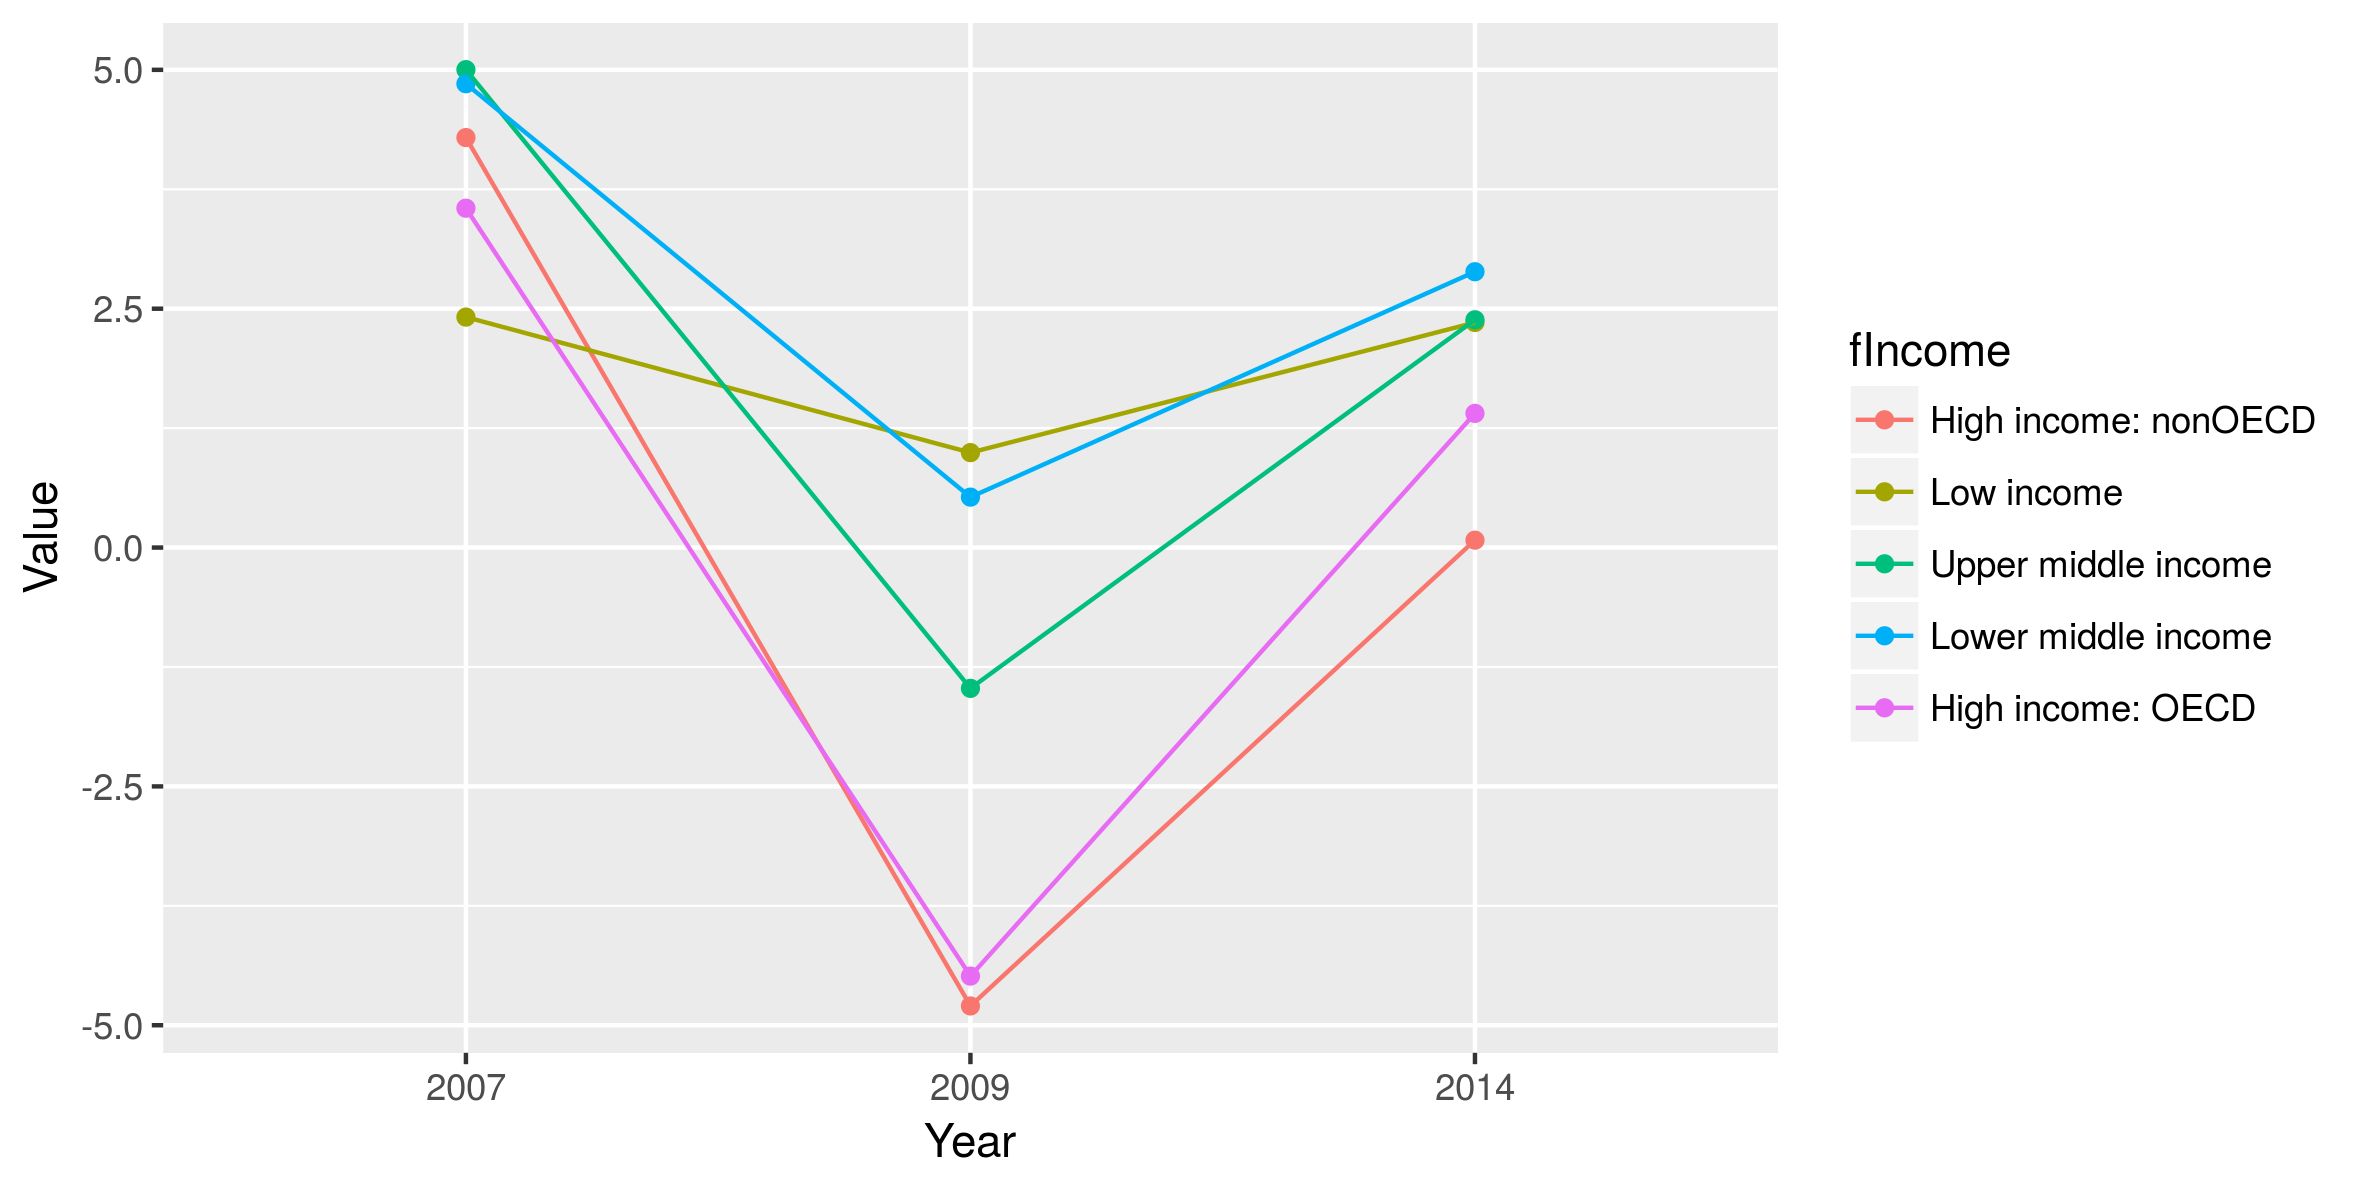
\includegraphics[height=3.5cm,width = 10cm]{Income2.png}
	\end{block}
\end{frame}











\end{document}